\section{Vorbereitung}
Die Versuchsvorbereitung ist Bestandteil des Versuchs. Sie erhalten dafür ein gesondertes Testat. Ohne
testierte Vorbereitung können Sie den Versuch nicht durchführen.
\subsection{Dioden}
\begin{enumerate}[label=\alph*)]
	\item Skizzieren Sie die Strom-Spannungskennlinie einer idealen Diode.
    \begin{figure}[h!]
      \begin{center}
        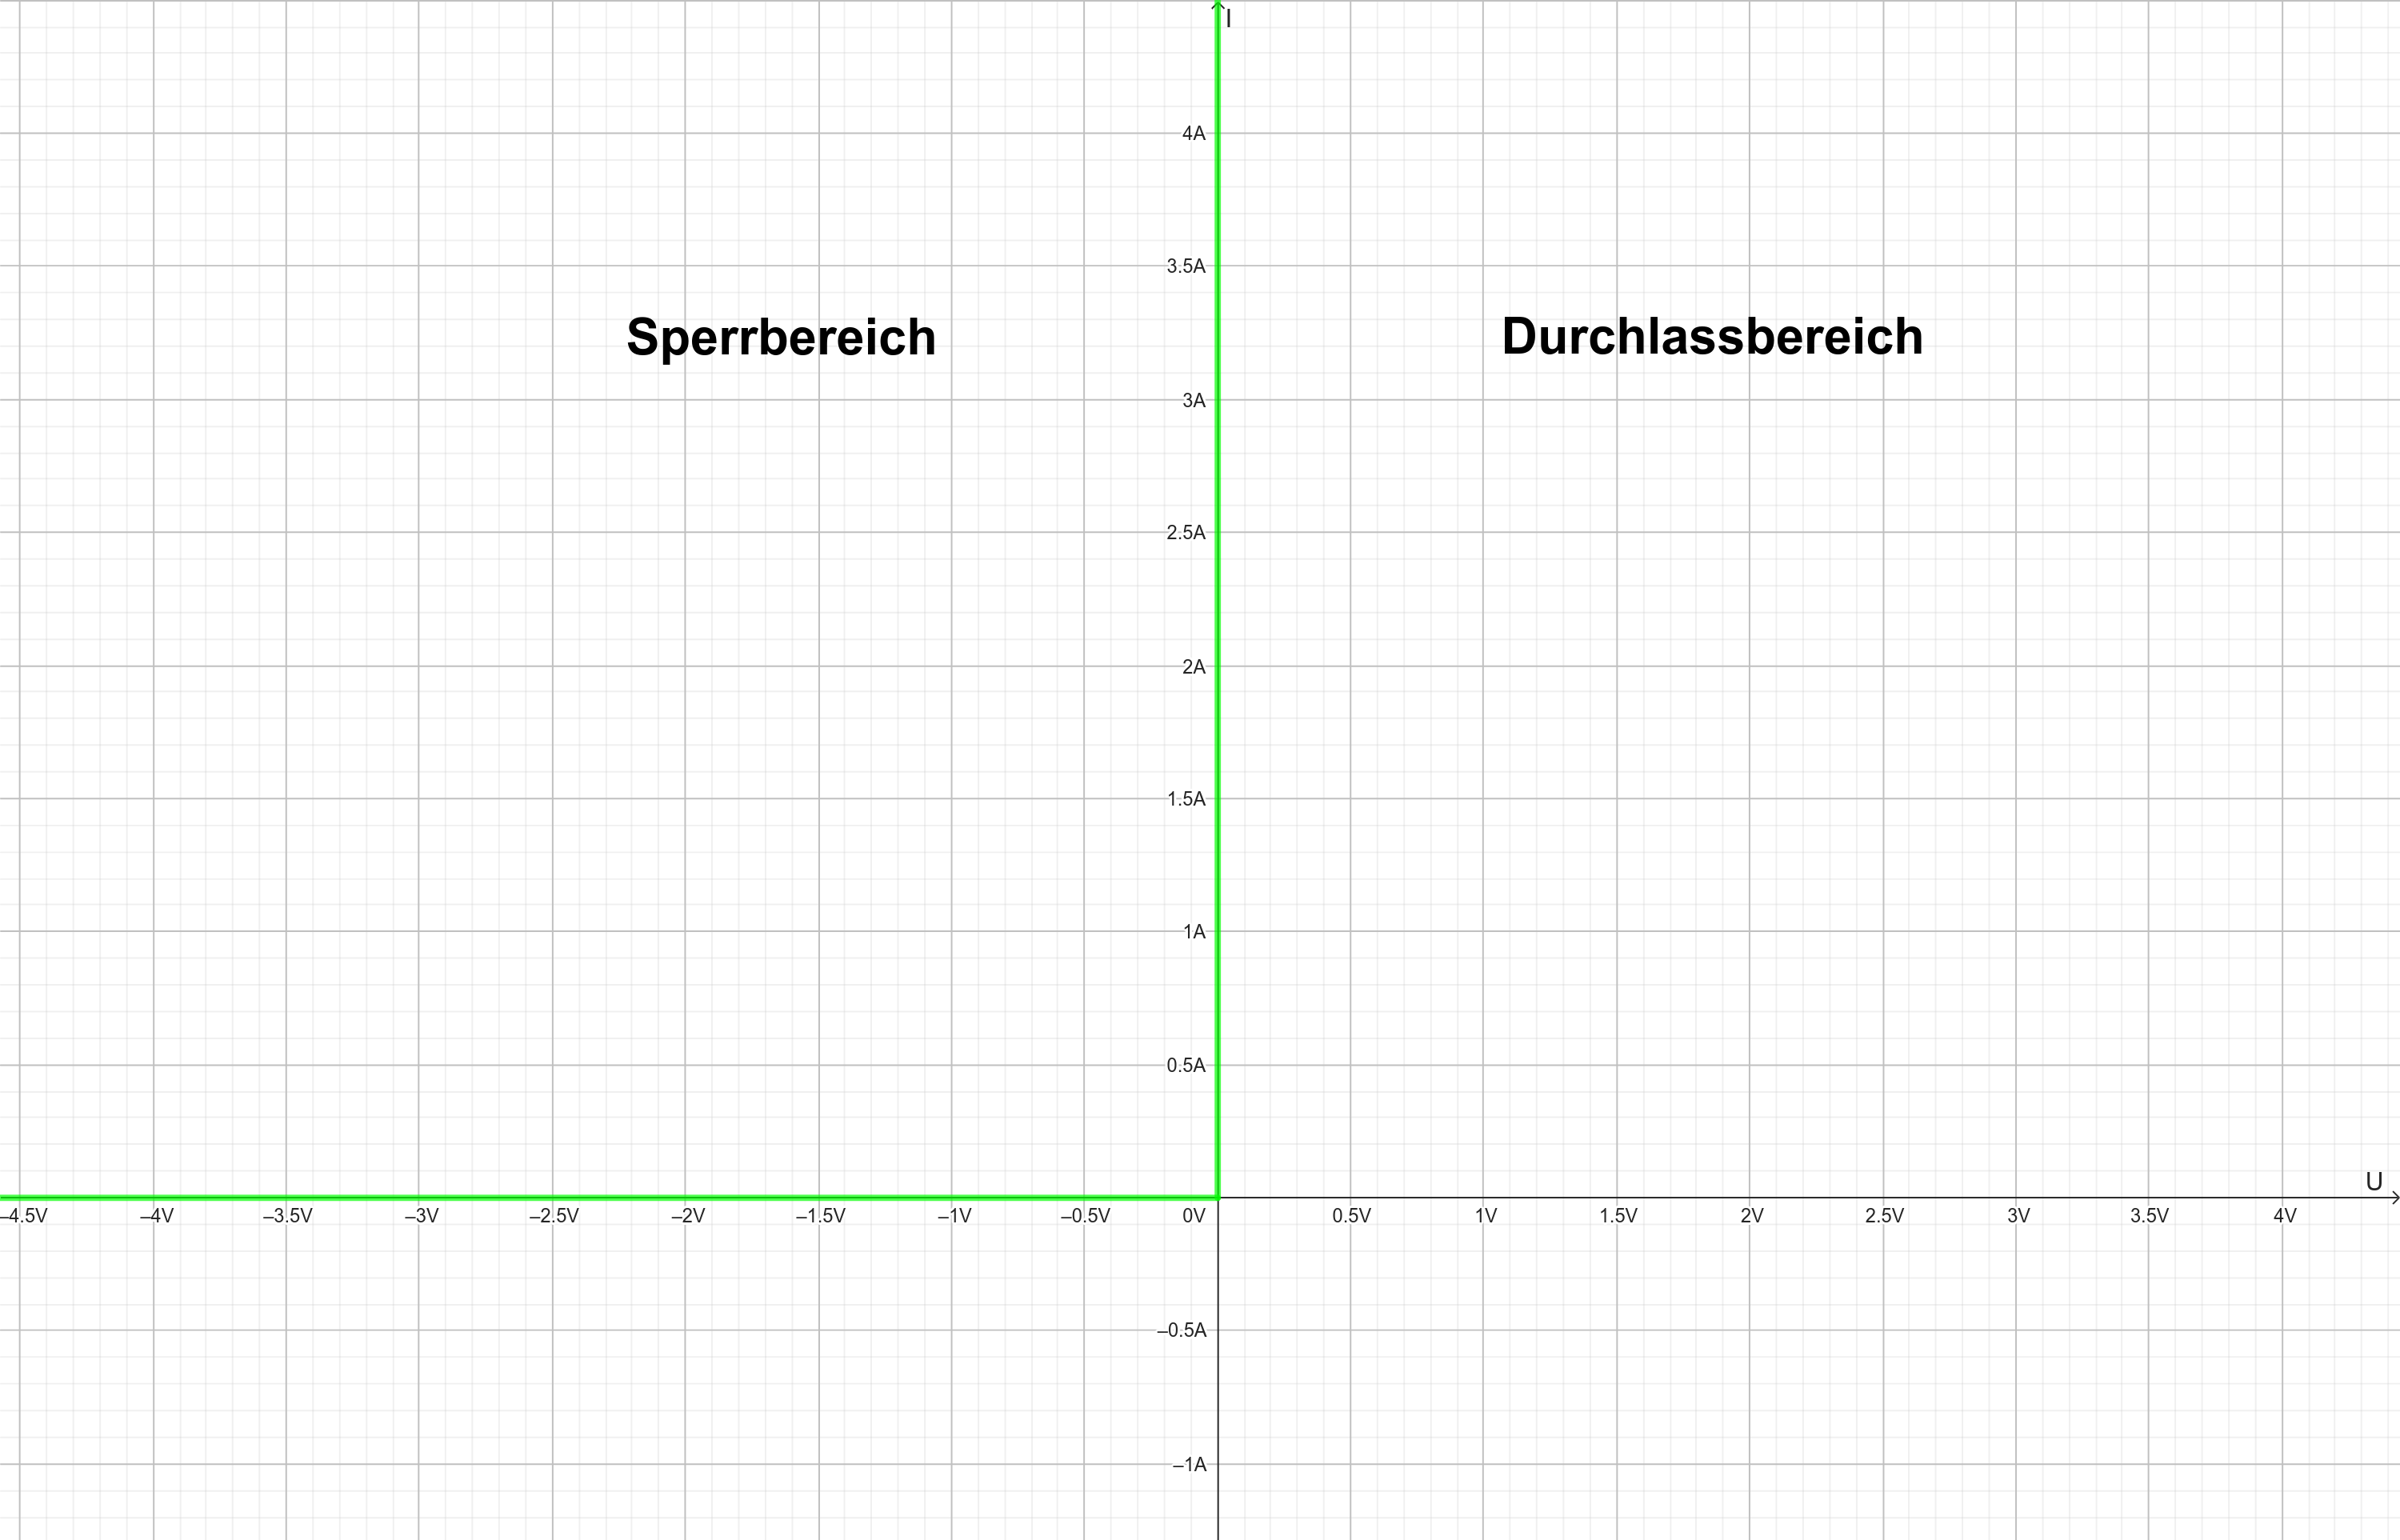
\includegraphics[width=0.6\textwidth]{img/2.1.1.1}
      \end{center}
      \caption{Strom-Spannungskennlinie einer idealen Diode}\label{img:2.1.1.1}
    \end{figure}
    
	\item Skizzieren Sie die Strom-Spannungskennlinie einer Leuchtdiode (LED 8MM RT von reichelt).
    \begin{figure}[h!]
      \begin{center}
        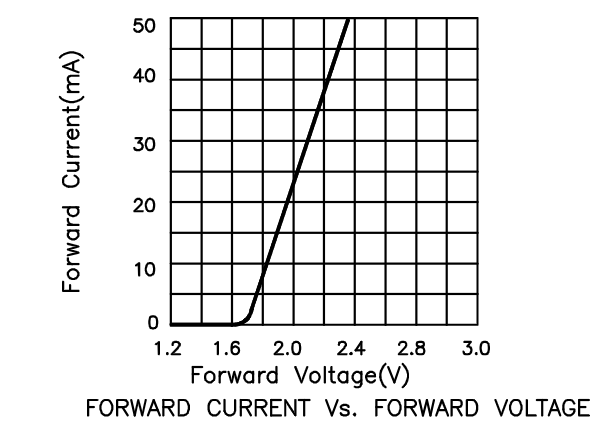
\includegraphics[width=0.6\textwidth]{img/2.1.2.1}
      \end{center}
      \caption{Strom-Spannungskennlinie von LED 8MM RT}\label{img:2.1.2.1}
    \end{figure}
    
	\item Diese Diode soll in Reihe mit einem Vorwiderstand an einer Spannungsquelle mit 3 V betrieben werden. Geben Sie das zugehörige Schaltbild an und bestimmen Sie grafisch den benötigten Widerstandswert.
    \begin{align*}
      R_v &= \frac{U_R}{I}\\
      R_v &= \frac{U - U_D}{I}\\
      R_v &= \frac{3\ V - 2\ V}{23\ mA}\\
    \end{align*}
	\item „3 Werte je Dekade im logarithmisch konstanten Abstand“ Was heißt das? Fertigen Sie dazu eine Skizze an.
    \begin{figure}[h!]
      \begin{center}
        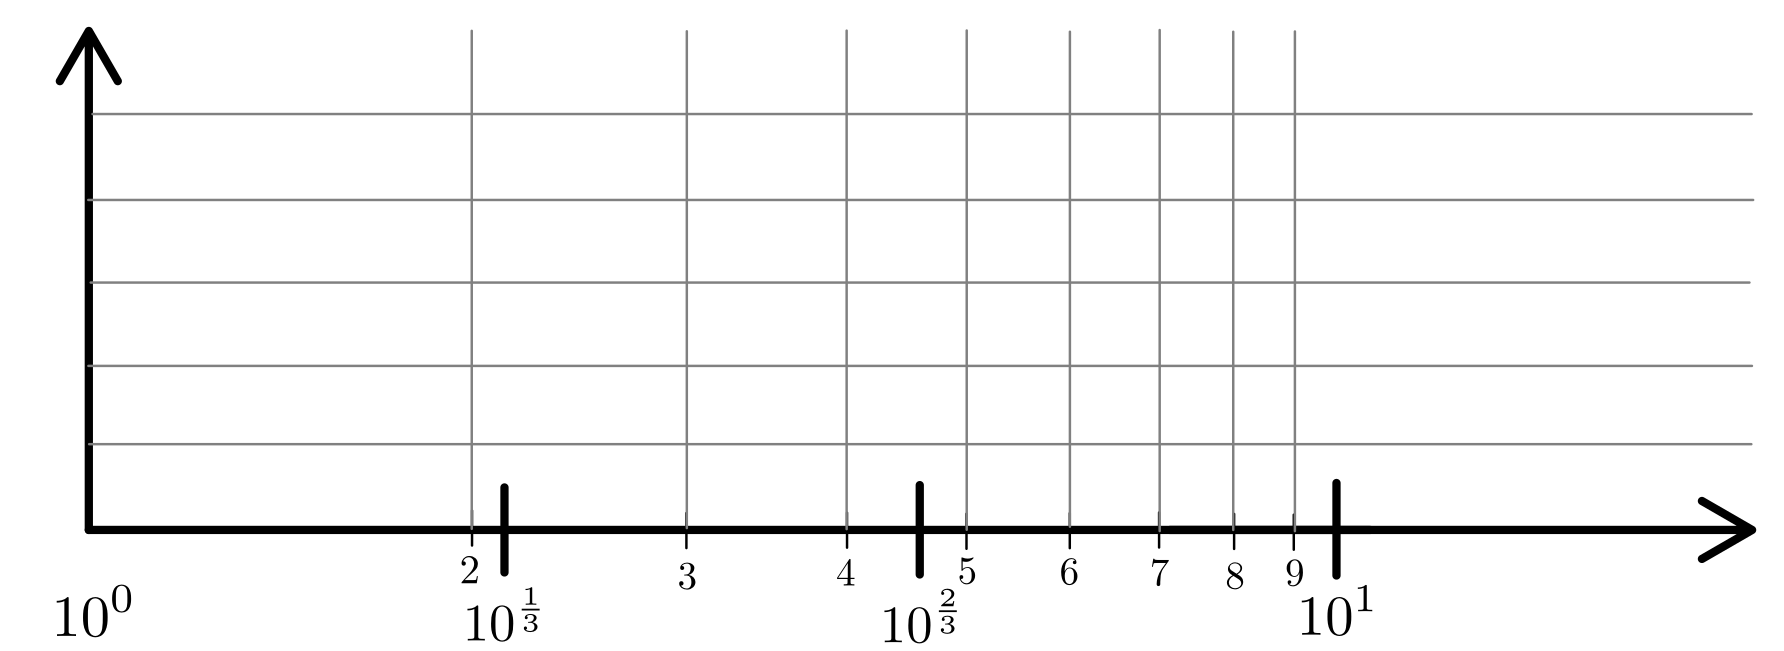
\includegraphics[width=0.75\textwidth]{img/2.1.4.1}
      \end{center}
      \caption{logarithmisch Skalierung}\label{img:2.1.4.1}
    \end{figure}
    
	\item Warum unterscheidet sich die Spannung an der Diode bei der Spannungsfehlerschaltung bei gleichem Strom in den unterschiedlichen Strommessbereichen?\\\ \\
    Für die unterschiedlichen Strommessbereichen hat das Messgerät unterschiedliche Innenwiderstände, deswegen verändert sich den Spannungsabfall an dem Messgerät.
	\item Wie müssen Sie den Strom bei der Stromfehlerschaltung korrigieren? Leiten Sie her!
    \begin{align*}
      I_{mess} &= I_x + I_U\\ 
      I_x &= I_{mess} - I_U\\ 
      I_x &= I_{mess} - \frac{U}{R_U}
    \end{align*}
	\item Bereiten Sie mit Excel oder einem vergleichbaren Programm Ihrer Wahl die Tabellen zur Aufnahme der Messwerte vor, so dass nach Eingabe der Messwerte die geforderten Diagramme automatisch erstellt werden. Werden nur Messwerte dargestellt, erfolgt die Darstellung als Linie mit Markierung (Kreuz, Dreieck, Quadrat) der Messwerte. Sollen in einem Diagramm der theoretische Verlauf und die Messwerte dargestellt werden, so wird der theoretische Verlauf als Linie mit mindestens 100 Stützwerten und die Messwerte mit Kreuz, Dreieck oder Quadrat markiert.
\end{enumerate}

\pagebreak
\subsection{Transistor}
\begin{enumerate}[label=\alph*)]
  \item Skizzieren Sie die Eingangskennlinie eines Transistors (BCY 59-8).
    \begin{figure}[h!]
      \begin{center}
        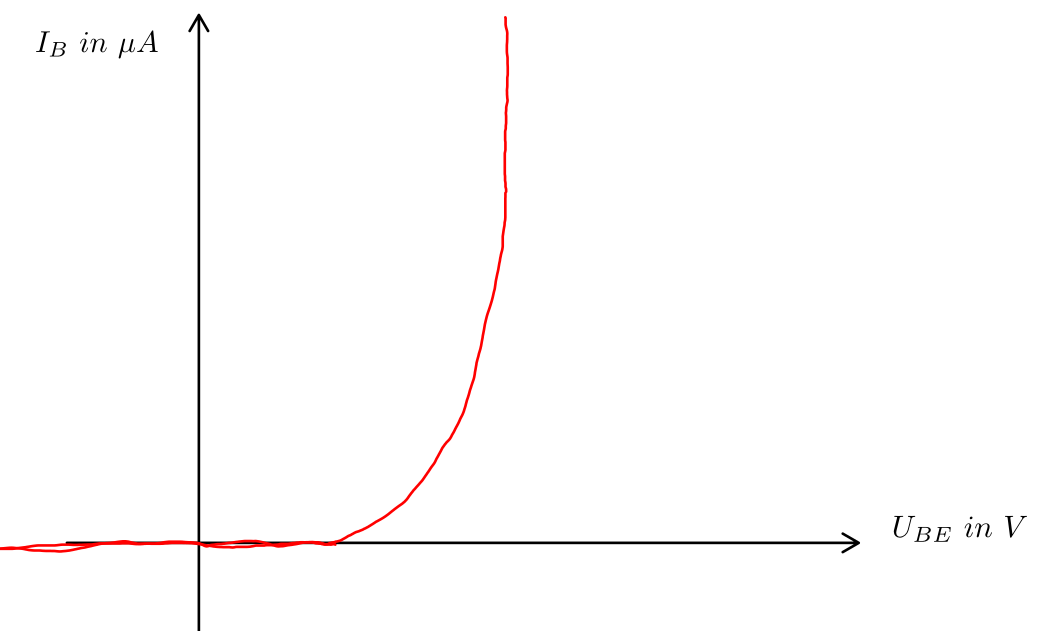
\includegraphics[width=0.4\textwidth]{img/2.2.1.1}
      \end{center}
      \caption{Eingangskennlinie eines Transistors}\label{img:2.2.1.1}
    \end{figure}
    
  \item Skizzieren die das Ausgangskennlinienfeld eines Transistors (BCY 59-8). 
    \begin{figure}[h!]
      \begin{center}
        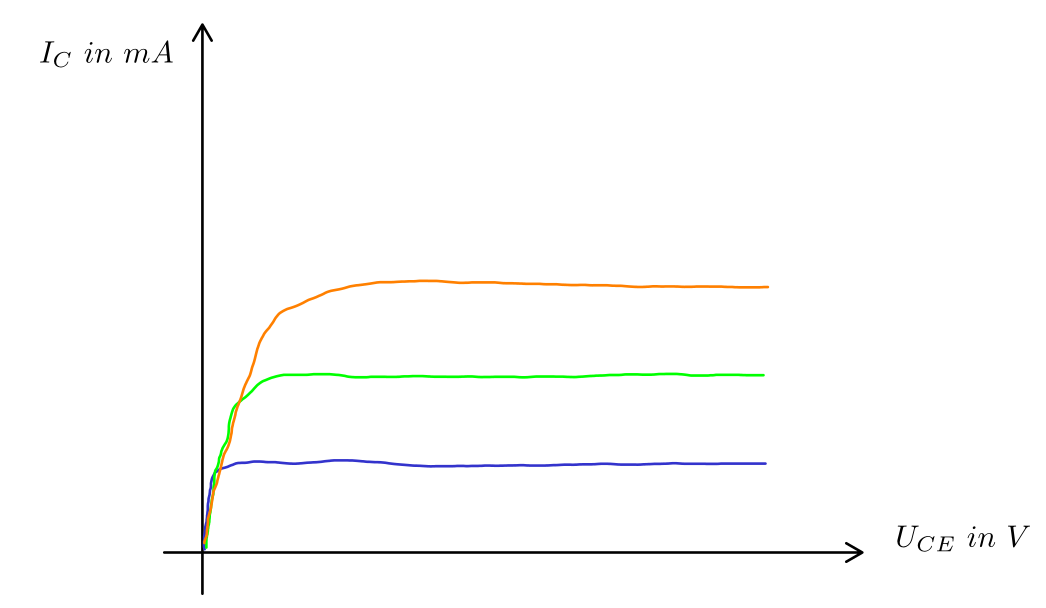
\includegraphics[width=0.4\textwidth]{img/2.2.2.1}
      \end{center}
      \caption{Ausgangskennlinie eines Transistors}\label{img:2.2.2.1}
    \end{figure}
    
  \item Welche Stromverstärkung hat dieser Transistor in etwa und wie kann sie aus den Messwerten ermittelt werden? \\
    $$h_{FE}=\beta = \frac{I_C}{I_B}$$
    \begin{figure}[h!]
      \begin{center}
        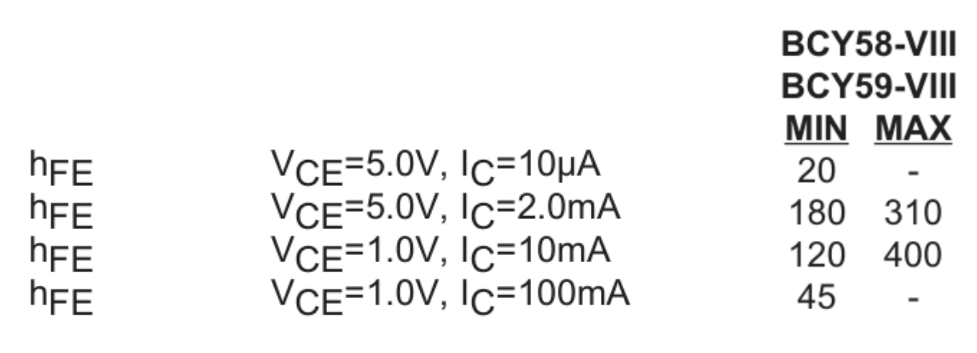
\includegraphics[width=0.5\textwidth]{img/2.2.3.1}
      \end{center}
      \caption{Stromverstärkung des Transistors}\label{img:2.2.3.1}
    \end{figure}
    
\pagebreak
  \item Bereiten Sie mit Excel oder einem vergleichbaren Programm Ihrer Wahl die Tabellen zur Aufnahme der Messwerte vor, so dass nach Eingabe der Messwerte die geforderten Diagramme automatisch erstellt werden. Werden nur Messwerte dargestellt, erfolgt die Darstellung als Linie mit Markierung (Kreuz, Dreieck, Quadrat) der Messwerte. Sollen in einem Diagramm der theoretische Verlauf und die Messwerte dargestellt werden, so wird der theoretische Verlauf als Linie mit mindestens 100 Stützwerten und die Messwerte mit Kreuz, Dreieck oder Quadrat markiert.  
\end{enumerate}
